% Created 2011-08-25 Thu 13:06
\documentclass[11pt,english]{article}
\usepackage[utf8]{inputenc}
\usepackage[T1]{fontenc}
\usepackage{fixltx2e}
\usepackage{graphicx}
\usepackage{longtable}
\usepackage{float}
\usepackage{wrapfig}
\usepackage{soul}
\usepackage{textcomp}
\usepackage{marvosym}
\usepackage{wasysym}
\usepackage{latexsym}
\usepackage{amssymb}
\usepackage{hyperref}
\tolerance=1000
\usepackage{color}
\usepackage{listings}

\usepackage{lmodern}
\renewcommand{\sfdefault}{lmss}
\renewcommand{\ttdefault}{lmtt}

% needed packages
\usepackage{amsmath}
\usepackage{amssymb}
\usepackage{amsthm}
\usepackage{babel}
\usepackage{epsfig}
\usepackage[T1]{fontenc}
\usepackage{fixltx2e}
\usepackage{float}
%\usepackage{floatflt}
\usepackage{graphics}
\usepackage{graphicx}
\usepackage[utf8]{inputenc}
\usepackage{latexsym}
\usepackage{longtable}
\usepackage{makeidx}
\usepackage{marvosym}
\usepackage{multicol}
%\usepackage{pslatex}
\usepackage{rotating}
%\usepackage{showidx}
\usepackage{soul}
\usepackage{srcltx}
\usepackage{stmaryrd}
\usepackage{subfig}
\usepackage{textcomp}
%\usepackage{theorem}
%\usepackage[subfigure]{tocloft}
\usepackage{txfonts}
\usepackage{upgreek}
\usepackage{url}
\usepackage{varioref}
%\usepackage{wasysym}
\usepackage{wrapfig}


% Page setup
\usepackage[paperwidth=8.5in,paperheight=11in]{geometry}
\geometry{verbose,tmargin=0.5in,bmargin=0.5in,lmargin=1in,rmargin=1in}




% PDF settings
%\usepackage[hyperref,x11names]{xcolor}
\usepackage{hyperref}
\hypersetup{pdftitle={STAT 5840: Statistical Computing},
 		pdfauthor={G. Jay Kerns}, 
		linkcolor=Firebrick4, 
		citecolor=black, 
		urlcolor=SteelBlue4}

% Listings setup
%\usepackage{color}
%\usepackage{listings}
%\lstset{basicstyle={\ttfamily},
%	language=R,
%	breaklines=true,
%	breakatwhitespace=true,
%	keywordstyle={\ttfamily},
%	numberstyle = {\ttfamily},
%	morestring=[b]"
%}



%  user defined commands
% special operators
\renewcommand{\P}{\mathrm{I\hspace{-1.5pt}P}}
\newcommand{\E}{\mathrm{I\hspace{-1.5pt}E}}
\renewcommand{\vec}[1]{\mbox{\boldmath$#1$}}

% special symbols
\newcommand{\me}{\mathrm{e}}
\newcommand{\R}{\mathbb{R}}
\newcommand{\diff}{\mathrm{d}}
\newcommand{\ybar}{\overline{y}}
\newcommand{\xbar}{\overline{x}}
\newcommand{\Xbar}{\overline{X}}
\newcommand{\Ybar}{\overline{Y}}





\providecommand{\alert}[1]{\textbf{#1}}

\title{Comparing Exponential and Lognormal Risks}
%\author{G. Jay Kerns}
\date{}

\begin{document}

\maketitle


\section*{Using Importance Sampling}
\label{sec-1}


We would like to compare risks of $X$ under an exponential $\mathrm{Exp}(\lambda)$ population versus a lognormal $\mathrm{Lnorm}(0,\sqrt{2}\log\,\lambda)$ population under the loss function
\[
L(\lambda) = \E \left[\frac{(X - \lambda)^{2}}{\lambda^{2}}\right].
\]
The following is a script to accomplish that goal.

\begin{verbatim}
# explognormal.R

# compute for a range of lambdas
lambda <- seq(from = 1.5, to = 10, by = 0.1)

m <- 100000                       # number of iterations (need a lot)
R1 <- rep(0, length(lambda))
R2 <- rep(0, length(lambda))

for (j in seq_along(lambda)){     # for each lambda, estimate risk
  l <- lambda[j]                  # get jth lambda
  sig <- sqrt(2*log(l))           # calc sigma
  x <- rlnorm(m, sdlog = sig)     # simulate m lognormals
  f1 <- l^(-1)*exp(-x/l)          # f1 is the exponential density
                                  # f2 is the lognormal density
  f2 <- (1/x)*(exp(-(log(x))^2/(2*sig^2)))/sqrt(2*pi*sig^2) 
  h <- (x - l)^2/l^2              # loss function
  R2[j] <- mean(h)                # lognormal risk
  R1[j] <- mean((h*f1)/f2)        # exponential risk
}
\end{verbatim}
\section*{At the command prompt}
\label{sec-2}



\begin{verbatim}
# now plot the results
par(mfrow = c(2,1))
plot(R1 ~ lambda, ylim = c(0,2), type = "l", main = "Exponential")
plot(R2 ~ lambda, ylim = c(0,60), type = "l", main = "Lognormal")
par(mfrow = c(1,1))
\end{verbatim}




\begin{figure}[h!]
\centering
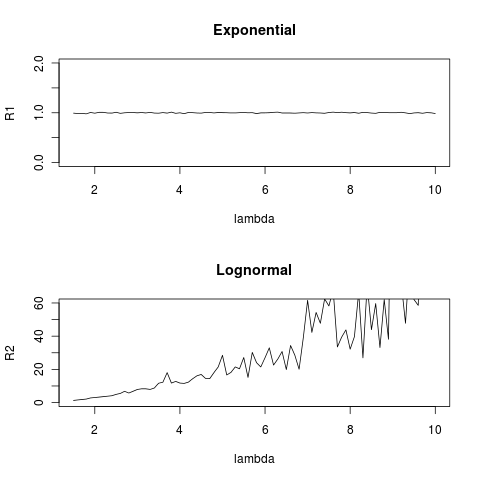
\includegraphics[width=7in, height=7in,]{img/ExpLognormal.pdf}
\caption{\label{fig:yplot}Risks at different values of $\lambda$ for the two populations.  We see that the risk for the exponential population is essentially constant while the risk for the lognormal population is sharply increasing in $\lambda$.}
\end{figure}

\end{document}